\capitulo{5}{Aspectos relevantes del desarrollo del proyecto}

\section{Metodologías Aplicadas}

Desde el inicio del proyecto se tenía muy claro que se iba a proceder de la manera más ordenada y profesional posible. Para poder realizar exitosamente este proceso recurrimos diferentes herramientas que nos permitiesen realizar un correcto desarrollo de este proyecto.
Fundamentalmente nos centramos en aplicar metodologías Ágiles.  Este concepto se podría definir como el conjunto de reglas y técnicas aplicadas a ciclos de trabajo de duración reducida. Esto permite tener una mayor flexibilidad durante el proyecto y una correcta entrega continua que nos permite la máxima colaboración con el cliente, en este caso el profesor Jesús Alberto San Martín Zapatero.
Debido a que la metodología ágil engloba a diferentes tipos de las mismas, a continuación se mencionan las usadas.
\begin{itemize}
    \item Kanban:
\end{itemize}
 La metodología Kanban consiste en poder informarte del estado de las tareas del proyecto de una forma visual y rápida, por lo que, con una rápida visualización, podemos saber el estado de cada una de las tareas existentes en el tablero.
 \begin{itemize}
     \item Scrum
 \end{itemize}
Esta metodología principalmente se posiciona en realizar ciclos de trabajos (Sprints) con una duración fija, en la que al finalizar se realiza una entrega del proyecto. 
En este caso se han realizado Sprints de 2 semanas con una reunión al finalizar el Sprint para poder debatir acerca de la entrega realizada y realizar las propuestas de trabajo para el siguiente Sprint.
Una vez generadas esas propuestas se transformaban en tareas que se incluían en el tablero Kanban para realizar un seguimiento a tiempo real del progreso del Sprint.
\begin{itemize}
    \item Lean
\end{itemize}
Esta metodología es posible que no sea tan frecuente como las dos anteriores, pero se fundamenta en la mejora continua y eliminar todos los lastres de tiempo posible en el proyecto. Esto permitía tener más tiempo para poder mejorar la calidad lo máximo posible al disponer de más tiempo para centrarnos en los detalles


\section{Inicio del proyecto}
Como primeros pasos para la integración del proyecto, se realiza un estudio para considerar el lenguaje que más se pudiera adaptar como se ha mencionado anteriormente como el Framework que nos pudiera permitir un desarrollo exitoso desde un inicio. De manera adicional, se determina como idea inicial obtener los datos a través de la realización de peticiones a una API de la que se obtuviese la información de los libros deseados.

Tras tomar esas decisiones iniciales, comienzo a investigar la estructura del Framework y los lenguajes HTML y CSS, ya que mi experiencia anterior con estas herramientas era muy limitada.

Una vez realizadas las investigaciones pertinentes, se genera un primer prototipo de página web con la estructura inicial y los elementos fundamentales. 
Antes de comenzar a trabajar con la API de Google, se crea una web básica con un sistema de gestión de libros utilizando una base de datos que permite realizar las siguientes operaciones de manera manual:

\begin{itemize}
    \item Barra de navegación que permite cambiar de página.
    \item Sistema de Login para gestionar la aparición de botones ocultos.
    \item Consultar todos los libros existentes en la base datos.
    \item Realizar búsquedas de los libros existentes en la base de datos en base al título o al ISBN.
    \item Agregar un libro a la base de datos.
    \item Editar un libro de la base de datos.
    \item Eliminar un libro de la base de datos.

\end{itemize}

El sistema de Login se estableció para no permitir que ningún usuario que no tuviese credenciales pudiera realizar modificaciones de la base de datos. En el caso de que ejecutaran la URL exacta de la función, la protección de seguridad les llevaría a la pantalla de Inicio de Sesión.

\begin{figure}[h]
    \centering
    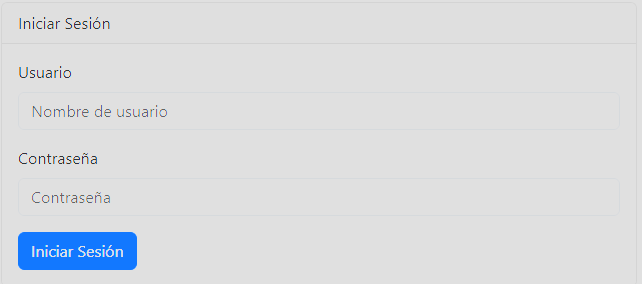
\includegraphics[width=0.9\textwidth]{Imagenes/Inicio_Sesion.png}
    \caption{Inicio de sesión}
    \label{fig:Inicio de sesión}
\end{figure}


\section{Desarrollo del proyecto}

Una vez presentado y debatido este primer prototipo de página web en el Sprint, se decide continuar de esta base agregando más elementos para añadirle funcionalidades. De manera adicional, se comienza a realizar un prototipo web para ir documentando el esquema de secciones existente en este proyecto. Tal como se comenta en la sección de Técnicas y Herramientas,  el prototipo web se realiza con el programa Justinmind.

Además, se agrega otra funcionalidad considerada como esencial, una página que al seleccionar el libro te muestre toda la información disponible en la base de datos para todo usuario interesado en obtener datos.
Para ello, en cada libro mostrado en el catálogo se pone a disposición un botón que te redirige a esta página.

Durante esa reunión se propone la idea de incluir un apartado especifico para los administradores que permite importar y exportar en un archivo CSV todos los datos de cada libro contenidos en la base de datos. 
Esta idea se concibe principalmente por dos grandes motivos
\begin{itemize}
    \item Tener la oportunidad de volcar datos más rápido desde el archivo CSV y posteriormente cargar el contenido del fichero en la base de datos.
    \item Poder tener un duplicado de la base de datos por si el contenido de la misma quedase inaccesible o se realizara un cambio indeseado, lo cuál se solucionaría restableciendo el catálogo con el archivo de seguridad descargado.

\end{itemize}
Aunque esta idea inicialmente funcionara. Al realizar pruebas se detectó un error durante la importación.
El error consistía en que un administrador pudiera colocar el signo "," para separar dos elementos como por ejemplo dos ISBN o que se encontrase en el contenido de la descripción del libro, lo cual generaba errores a la hora de transformar los campos a columnas al tener ese mismo signo como delimitador. Por ese motivo se propuso la idea de cambiar el delimitador por defecto a el signo ";".

Tras realizar estas correcciones de errores iniciamos el proceso de obtener la información  de los libros de forma automática Aunque de manera inicial se valoró la opción de utilizar únicamente la API de Google Books,  se consideró interesante para  dar más fuentes de información y aumentar la dificultad técnica del proyecto la utilización de Web scraping. 
El  web scraping realizado se aplicó sobre 2 páginas web las cuales tienen un catálogo de libros muy amplio. Estas webs son \href{https://www.amazon.es/}{Amazon} y \href{https://www.agapea.com/}{Agapea}. Estos tres proveedores nos permiten que en base a un ISBN o un Título, internamente se lancen unos procesos que busquen en los proveedores con las diferentes técnicas mostradas para que se pueda seleccionar el proveedor que nos de la información más precisa. 
En el caso de que se quisiera agregar un libro automáticamente pero se desee personalizar y usar una mezcla de los 3 proveedores, se dispone de un sistema de desplegables que nos permite realizar esta acción.

Durante el desarrollo en este espacio de tiempo, se considera que sería necesario implementar un sistema que nos permitiese proteger el catálogo de una importación que pueda encontrarse corrupta o con datos erróneos.
Por lo que antes de realizar la importación, aparece una ventana modal que recuerda al usuario que debería de exportar el catálogo actual por seguridad.